\documentclass[12pt, oneside]{book}
\usepackage[spanish]{babel}
\usepackage{geometry}
\usepackage[utf8]{inputenc}
\usepackage{amsmath}
\usepackage{amssymb} 
\usepackage{amsthm}
\usepackage{xcolor}
\usepackage{algorithm}
\usepackage{algorithmic}
\usepackage{graphicx}

\newtheorem*{definition}{Definición}
\newtheorem*{proposition}{Proposición}
\newtheorem*{theorem}{Teorema}
\newcommand{\norm}[1]{\left\lVert#1\right\rVert}
\renewcommand{\proofname}{Demostración}

\title{Algunos métodos iterativos (e implementaciones) para la solución de problemas inversos discretos}
\author{}
\date{}

\begin{document}
	\maketitle
	\tableofcontents
	
	
	\chapter{Métodos Iterativos para resolver problemas inversos}
	\ En este texto se pretende estudiar el problema de enfoque de imágenes. A partir de una imagen borrosa con ruido y una matriz de desenfoque, nuestro objetivo es encontrar nuestra imagen original utilizando su versión borrosa. Este problema se puede formular a través de un sistema lineal $Ax = b$, donde $A$ es la matriz de desenfoque, $b$ es el ruido y $x$ es la imagen a restaurar. Debido a su mal condicionamiento, nos interesan los métodos de regularización para la reconstrucción de las mismas. En particular, nos interesaremos por los métodos iterativos de Krylov. Estos métodos están basados en procesos de proyección sobre un tipo de subespacios muy particulares, de los cuales el método toma el nombre. Este capítulo servirá de introducción a la estructura general de esta clase de métodos.
	
	Con el fin de ejemplificar los métodos mostrados y ver sus respectivas implementaciones, trabajaremos como ejemplo con la siguiente imagen de $64\times 64$ pixeles.
	
	\begin{figure}[H]
		\centering
		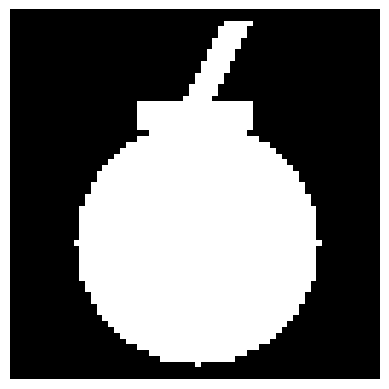
\includegraphics[scale=0.5]{Imagenes/x_true.png}
		\caption{Imagen de un mate, la cual usaremos para ejemplificar.\\}
	\end{figure}
	
	El ruido por lo general no tiene una forma especifica, y con fines de replicar un problema lo mas fidedigno a la realidad, se debe aplicar un tipo de ruido de acuerdo al problema que se quiere estudiar. Entre los tipo de ruidos mas comunes encontramos el Gaussiano, el de Poisson, el de Laplace, y el de Salt\&Pepper. A lo largo de este trabajo asumimos el ruido del primer tipo. 
	
	\begin{figure}[H]
		\centering
		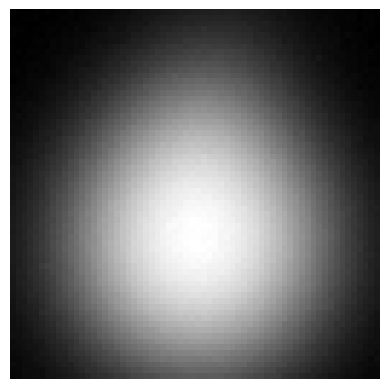
\includegraphics[scale=0.3]{Imagenes/mate_Gauss.png}
		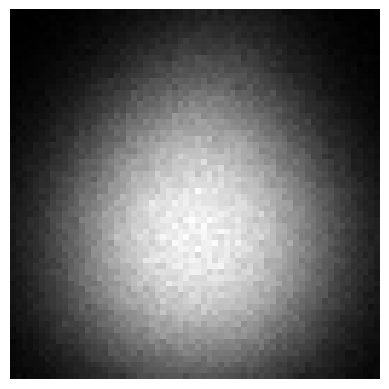
\includegraphics[scale=0.3]{Imagenes/mate_Poisson.png}
		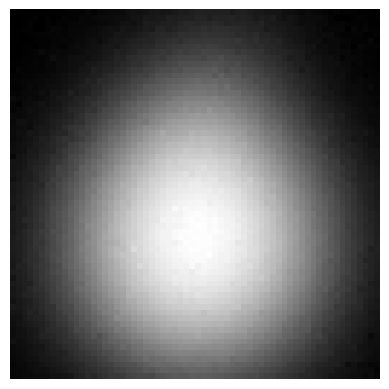
\includegraphics[scale=0.3]{Imagenes/mate_Laplace.png}
		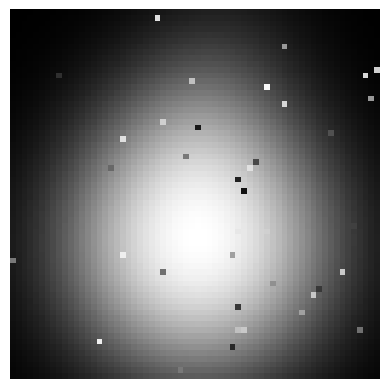
\includegraphics[scale=0.3]{Imagenes/mate_saltpepper.png}
		\caption{De izquierda a derecha: Ruido Gaussiano, ruido de Poisson, ruido de Laplace, ruido Salt\&Pepper\\}
	\end{figure}
	
\section{Métodos Iterativos}

Consideremos el problema lineal dado por el sistema $Ax = b$. Sabemos que existen métodos directos para la resolución de los mismos (descomposiciones QR, de Cholesky, PALU, entre otros), pero estos métodos traen consigo limitaciones. El primer obstáculo que nos podemos encontrar viene con la cantidad de operaciones que requieren y el tiempo computacional que inducen cuando la matriz $A$ sube de dimensión, la estructura que puede tener o incluso no tenerla de forma explícita y que venga en forma de operador lineal o función.

A raíz de estas limitaciones con los métodos directos, surgen los métodos iterativos. La idea es que dado un sistema $Ax = b$ y un vector inicial $x_0$, el método produce una sucesión $\{x_n\}_{n \in \mathbb{N}}$ de soluciones del sistema que, dadas las condiciones necesarias, convergen a $x$.

Para plantear un método, dado el sistema lineal y la matriz $A$, la reescribimos como $A=M+N,$ lo que nos deja con el sistema: $$(M-N)x=b,$$ 
el cual se traduce a: $$Mx=b+Nx.$$
Y si resolvemos para $x$ tenemos que: $$x=M^{-1}(b+Nx).$$ 
De donde podemos deducir la fórmula recursiva de método $$x_{n+1}=M^{-1}(b+Nx_{n}).$$
Ademas, teniendo en cuenta que $N=M-A$, concluimos que $$x_{n+1}=M^{-1}(b+(M-A)x_{n})=M^{-1}b+x_n-M^{-1}Ax_n.$$ 
Luego, $$x_{n+1}=x_n+M^{-1}(b-Ax_n),$$ 
la cual es la fórmula general para cualquier método iterativo.

Pero habíamos dicho que para asegurar que la sucesión $\{x_n\}_{n \in \mathbb{N}}$ generada por el método resultase convergente necesitábamos que se den ciertas condiciones, vamos a verlas a continuación.

\subsubsection{Error de los métodos}
\ Partiendo de la forma del método: $$x=M^{-1}b+(I-M^{-1}A)x$$ Tenemos que la forma iterativa viene dada por: $$x_{n+1}=M^{-1}b+(I-M^{-1}A)x_n$$ Y entonces tenemos que la diferencia entre iteraciones nos da el error del paso $n+1$: $$e_{n+1}=(I-M^{-1}A)e_n$$ Entonces si llamamos $B=I-M^{-1}A$ tenemos que: $$e_{n+1}=Be_n=BBe_{n-1}=\dots=B^{n+1}e_0$$ Y por lo tanto tenemos que: $$\norm{e_{n+1}} \leq \norm{B}^{n+1}\norm{e_0}$$

\ Notemos que si $\norm{B}<1$, entonces $\norm{e_n}\xrightarrow{n \xrightarrow{} \infty}0$.


\subsection{Métodos estándar}
Habíamos quedado en que un método iterativo viene dado por la fórmula recursiva $$x_{n+1}=x_n+M^{-1}(b-Ax_n).$$ Pero para poder hacer esto, necesitábamos descomponer nuestra matriz $A$ y toda la iteración iba a depender de eso.

Dado un sistema lineal, podemos descomponer a su matriz $A$ como $A=L+D+U$, con $L$ su parte triangular inferior estricta, $D$ su diagonal y $U$ como su parte triangular superior estricta. Y tenemos que $$Ax=b \iff Dx=-(L+U)x+b \iff (L+D)x=-Ux+b$$ Con esto podemos definir los dos métodos iterativos más comunes.
\subsubsection{Método de Jacobi}
Sabiendo que $Dx=-(L+U)x+b$, podemos escribir la forma recursiva como: $$Dx_{n+1}=-(L+U)x_n+b$$ Y esto nos dice que: $$x_{n+1}=-D^{-1}(L+U)x_n+D^{-1}b$$ Y esta es la iteración del método de Jacobi.
\subsubsection{Método de Gauss-Seidel}
Partiendo de que $(L+D)x=-Ux+b$ es equivalente al sistema $Ax=b$, vemos que su forma recursiva está dada por: $$(L+D)x_{n+1}=-Ux_n+b$$ Y esto lo podemos reescribir como: $$x_{n+1}=-(L+U)^{-1}Ux_n+(L+U)^{-1}b$$ Que es la iteración del método de Gauss-Seidel.

\ En general, podemos decir que las iteraciones de los métodos vienen dadas por $x_{n+1}=Bx_n+C$, y en el caso de Jacobi, $B_J=-D^{-1}(L+U)$ y $C_J=D^{-1}b$ y para Gauss-Seidel $B_{GS}=-(L+U)^{-1}U$ y $C_{GS}=(L+U)^{-1}b$.

Sin embargo, la deficiencia de estos métodos radica en que son muy costosos computacionalmente. De ahí su inviabilidad para implementarlos incluso para matrices no muy grandes. Este problema, en cierta medida, motiva el estudio de métodos iterativos que son esencialmente distintos en su implementación y que requieren de su propia teoría. Uno de estos métodos son los basados en los subespacios de Krylov. 

\subsection{Métodos de Krylov}
\begin{definition}
	Dada $A$ una matriz y $v, Av, \dots , A^{m-1}v \in \mathbb{C}^m$ vectores linealmente independientes, llamamos subespacio de Krylov de dimensión $m$ a: $$\mathcal{K}_{m}(A, v) = \langle v, Av, \ldots, A^{m-1}v \rangle$$
\end{definition} 
\ Los métodos de Krylov son métodos iterativos que utilizan subespacios de Krylov que, dado $x_0$ una aproximación inicial de la solución del sistema, se define el subespacio $\mathcal{K}_{m}(A, r_0)$, con $r_0=b-Ax_0$.

\ Para entender de donde surge la idea de utilizar subpesacios de Krylov, notemos que dado la solución $x_{true}=A^{-1}b$ y $x_0$ una aproximación inicial para el método, resolver el sistema original es equivalente a resolver $Az=r_0$ si $z=x_{true}-x_0$. Sea $p(x)$ el polinomio de menor grado $i$ tal que $p(A)r_0=0$. Por el teorema de Cayley-Hamilton, tenemos que $i\leq n$. Entonces tenemos que: $$p(A)=a_0+Aa_1+\dots+a_{i-1}A^{i-1}+a_iA^i=0.$$ Por lo que vale que $$A^{-1}a_0=-(a_1I+a_2A+\dots+a_{i-1}A^{i-2}+a_iA^{i-1})$$ Y si multiplicamos por $r_0$ tenemos que: $$z=A^{-1}r_0=-\frac{1}{a_0}(a_1I+a_2A+\dots+a_{i-1}A^{i-2}+a_iA^{i-1})r_0$$ Por lo que $$z\in \langle r_0,Ar_0,\dots,A^{i-1}r_0 \rangle = \mathcal{K}_{m}(A, r_0)$$ o bien, $$x_{true} \in x_0 + \mathcal{K}_{m}(A, r_0).$$

Así nos podemos convencer que la formulación de un subespacio de Krylov para resolver sistemas lineales sale naturalmente de entender el problema.

\subsection{Metodos de Proyección}

Debido a la gran escala de las matrices y su mal condicionamiento, estos sistemas se suelen resolver a través de la proyección a subespacios de Krylov dimensión más pequeña. 

En el apartado anterior, vimos que la solución $x$ está contenida en el subespacio afín $x_0 + \mathcal{K}_m(A, r_0)$. Naturalmente, esto nos lleva a pensar que la solución $x_n$ puede ser computada en el subespacio $x_0 + \mathcal{K}_n(A, r_0)$. Equivalentemente,
\begin{center}
	$x_n = x_0 + y_n, \quad  y_n \in \mathcal{K}_n(A, r_0)$
\end{center}
para $n \in \mathbb{N}$. Nuestro objetivo es encontrar la mejor combinación lineal de coeficientes para el subespacio de Krylov, con el fin de que a partir de una cierta iteración $m$, se obtenga la solución exacta (o suficientemente aproximada).

Sea $x_0 \in \mathbb{C}^n$ un vector inicial y sea $r_0 := b - Ax_0$. El residuo correspondiente a la iteración $n$ está dado por:
\begin{center}
	$r_n := b - Ax_n = b - A(x_0 + y_n) = r_0 - Ay_n, \quad r_n\in \ \mathcal{K}_{n+1}(A, r_0)$
\end{center}
Para poder determinar la solución $x_n$ de manera óptima, se imponen ciertas restricciones, que suelen describir a partir de nociones de ortogonalidad. Estos son algunos de los enfoques:

\begin{flushleft}
	\textbf{Enfoque de Ritz-Galerkin}
\end{flushleft}
Para cada $n \in \mathbb{N}$, pedimos
\begin{center}
	$r_n \perp \mathcal{K}_{n}(A, r_0).$
\end{center}
\begin{flushleft}
	\textbf{Enfoque de Petrov-Galerkin}
\end{flushleft}
Para este enfoque, pedimos que el residuo (definido previamente) sea ortogonal a un subespacio $\mathcal{L} \subset \mathbb{C}^{n}$ de dimensión $n$, es decir,
\begin{center}
	$r_n \perp \mathcal{L}_n$, con $dim(\mathcal{L}_n) = n$
\end{center}
\newtheorem{proposicion}{Proposición}
\begin{proposicion}
	El enfoque de Ritz-Galerkin es el enfoque de Petrov-Galerkin con la elección $\mathcal{L}_n = \mathcal{K}_{n}(A, r_0)$.
\end{proposicion}
Para poder representar este problema matricialmente, consideramos V = $[v_1, \ldots, v_m]$ y W = $[w_1, \ldots, w_m]$, cuyas columnas definen bases de $\mathcal{K}$ y $\mathcal{L}$ respectivamente. La solución aproximada $\tilde{x}$ ahora puede ser escrita como $\tilde{x} = x_0 + Vy, \quad y \in \mathbb{C}^n$. Si definimos $r := b - A\tilde{x}$, para que éste sea ortogonal a $\mathcal{L}$ pedimos:
\begin{center}
	$W^Tr = 0 \iff W^T(b - A\tilde{x}) = 0 \iff W^T(b - A(x_0 + Vy)) = 0 \iff \boxed{W^TAVy = W^Tr_0}$.
\end{center}
Si $W^TAV$ es invertible, entonces la aproximación está dada por:
\begin{center}
	$\tilde{x} = x_0 + V(W^TAV)^{-1}W^Tr_0$
\end{center}

\subsection{Arnoldi}

A veces es útil hallar una base orto-normal para un método iterativo, pues uno espera que de esta forma se elimine 'información redundante' ahorrando así costo computacional. Una manera de hallar una base orto-normal en un espacio de Krylov $\mathcal{K}_m$ es con el método de Arnoldi.
	
	\begin{algorithm}
		\caption{Arnoldi}
		\begin{algorithmic}[1]
			\STATE Comenzamos con $v_1 = \frac{v}{\|v\|}$.
			\FOR{$j \in \{1, 2, \dots, i\}$} 
				\STATE Computamos $h_{ij} = v_i^TAv_j$ para $i \in \{1, 2, \dots, j\}$
				\STATE $w_j = Av_j - \sum_{i=1}^j h_{ij} v_i$
				\STATE $h_{j+1,j} = \|w_j\|_2$
				\STATE \textbf{if} $h_{j+1,j} = 0$ \textbf{then} Stop
			\ENDFOR
			\STATE $v_{j+1} = w_j / h_{j+1,j}$
		
		\end{algorithmic}
	\end{algorithm}
	
	Si denotamos a $V_i$ a la matriz de tamaño $n\times i$ que tiene a los vectores $v_1, ..., v_i$ como columnas, a $H_i$ como la matriz de Hessemberg de tamaño $(i+1)\times i$ cuyos elementos no nulos son los $h_{ij}$ descritos en el algoritmo de Arnoldi, entonces se verifica que $$AV_j=V_{j+1}H_i.$$
	
	Donde la matriz de Hessemberg es de la forma: 
	
	$$
	\mathbf{H_m} =
	\begin{bmatrix}
		h_{11} & h_{12} & h_{13} & \cdots & h_{1m} \\
		h_{21} & h_{22} & h_{23} & \cdots & h_{2m} \\
		0      & h_{32} & h_{33} & \cdots & h_{3m} \\
		\vdots & \ddots & \ddots & \ddots & \vdots \\
		0      & \cdots & 0      & h_{m-1,m} & h_{mm}
	\end{bmatrix}
	$$
	
	
\subsection{GMRES}
	Una forma novedosa de resolver un sistema lineal usando métodos iterativos, es intentar minimizar la norma de un vector residual, donde se define un residuo inicial $r_0=b-Ax_0$ y se busca $x$ de modo que se minimice $J(y)=||b-Ax||_2$.
	
	El método GMRES (Generalized Minimal Residual Method) aprovecha esta idea, minimizando en cada paso un vector residual proyectado sobre un subespacio de Krylov a través de sus componentes orto-normales. 
	
	Para deducir el método, hagamos un par de observaciones.
	
	Consideremos $\mathcal{K}_m=\mathcal{K}_{m}(A, r_0)$ y un vector inicial $x_0$. luego cualquier vector en $x_i\in\mathcal{K}_m+x_0$ se escribe como $$x=x_0+V_my.$$
	Donde $V_m$ es la misma matriz definida en el método de Arnoldi, e $y$ es un vector de tamaño $m$. Sean $\beta = ||r_0||_2$ y $v_1=\frac{r_0}{||r_0||_2}$, y teniendo en cuenta la igualdad en el método de Arnoldi, podemos reescribir el problema a minimizar como:
	\begin{equation*}
		\begin{split}
			b-Ax&=b-A(x_0+V_my)\\
			    &= r_0-AV_my\\
			&= \beta v_1-V_{m+1}H_my\\
			&= V_{m+1}(\beta e_1 - H_my).
		\end{split}
	\end{equation*}
	Luego 
	\begin{equation*}
		\begin{split}
			J(y)&=||b-Ax_i||_2\\
			&=||V_{m+1}(\beta e_1 - H_my_m)||_2    
		\end{split}
	\end{equation*}
	y como los vectores columna de $V_{m+1}$ son orto-normales, entonces:
	$$J(y)=||\beta e_1 - H_my||_2.$$
	
	Entonces el problema se reduce a resolver un problema de mínimos cuadrados de tamaño $(m+1)\times m$, que es menos demandante computacionalmente que el problema original. El poder de GMRES reside en que bajamos la dimensión del problema original considerablemente, sin embargo el algoritmo no provee una solución explicita en cada paso, sino que hace falta calcularla en intervalos regulares. (En realidad hay varias formas de resolver esta deficiencia del algoritmo, pero no es el objetivo de este trabajo. Una fuente donde se desarrolla mejor esta idea es en el libro Iterative Methods de Yousef Saad).
	
	\begin{algorithm}
		\caption{Algoritmo GMRES}
		\begin{algorithmic}[1]
			\STATE \textbf{Dada} $\mathbf{A} \in \mathbb{R}^{n \times n}$, $\mathbf{b} \in \mathbb{R}^n$, $\mathbf{x}^{(0)}$, calcular $\mathbf{r}^{(0)} = \mathbf{b} - \mathbf{A} \mathbf{x}^{(0)}$
			\STATE $\mathbf{v}_1 = \frac{\mathbf{r}^{(0)}}{\|\mathbf{r}^{(0)}\|}$
			\FOR{$k = 1, 2, \dots, m$}
			\STATE Calcular $\mathbf{w_k} = \mathbf{A} \mathbf{v}_k$
			\FOR{$j = 1, \dots, k$}
			\STATE $h_{jk} = \mathbf{w}^T \mathbf{v}_j$
			\STATE $\mathbf{w_k} := \mathbf{w_k} - h_{jk} \mathbf{v}_j$
			\ENDFOR
			\STATE $h_{k+1,k} = \|\mathbf{w_k}\|$
			\IF{$h_{k+1,k} \neq 0$}
			\STATE $\mathbf{v}_{k+1} = \frac{\mathbf{w_k}}{h_{k+1,k}}$
			\ENDIF
			\ENDFOR
			\STATE Resolver el problema de mínimos cuadrados $\min_y \|\beta \mathbf{e}_1 - \mathbf{H}_k y\|_2$
			\STATE Actualizar la solución: $\mathbf{x}^{(k)} = \mathbf{x}^{(0)} + \mathbf{V}_k y$
			\IF{$\|\mathbf{r}^{(k)}\| <$ tolerancia}
			\STATE Romper el ciclo
			\ENDIF
		\end{algorithmic}
	\end{algorithm}
	
	Aplicando este método a nuestro ejemplo inicial, y aplicando un criterio de tolerancia en el residuo, obtenemos una reconstrucción bastante decente. La figura es distinguible, a pesar de que aun la reconstrucción es bastante insatisfactoria.
	\begin{figure}[H]
		\centering
		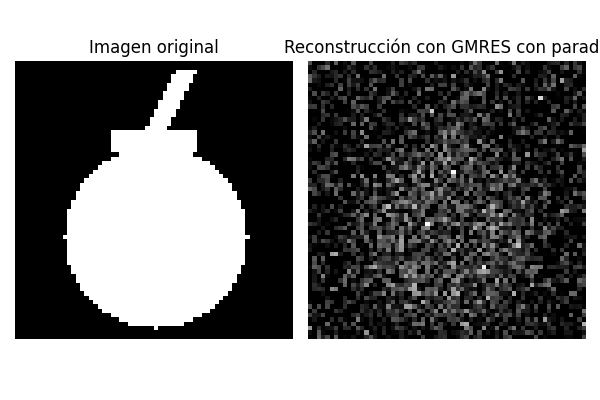
\includegraphics[scale=0.5]{Imagenes/mate_GMRES.png}
		\caption{Reconstrucción de la imagen con ruido usando GMRES.\\}
	\end{figure}

\subsection{Otros métodos.}

Si bien hemos desarrollado la teoría para llegar a GMRES, los espacios de Krylov dan lugar a otros métodos que se basan en las mismas ideas. 
 A breves rasgos, la iteracion de un metodo de Krylov debe cumplir lo siguiente
 $$x^{(k)} \in \underset{x \in \mathcal{K}_m(A, v)}{\mathrm{arg\,min}} \, \|\mathcal{F}(x)\|
 $$ 
 donde $\mathcal{F}$ es la funcion con argumento $x$ que nos interesa minimizar iterativamente, proyectando en el subespacio $\mathcal{K}_m(A,v)$.
 
 En estas ideas se basan LSQR y LSMR, donde ambos se sobre el subespacio de Krylov $\mathcal{K}_m (AA^t, r_0)$, aunque minimizan una $F(x)$ distinta. A saber: LSQR minimiza el problema de minimos cuadrados $||Ax-b||$, mientras que LSMR resuelve el problema regularizado $||(A^tA+\lambda ^2 I)x-A^tb||$.

Las ventajas de estos enfoques son que son mas estables computacionalmente para problemas contaminados con ruido. En nuestro caso, la mejora es significativa con respecto al método anterior. 

\begin{figure}[H]
	\centering
	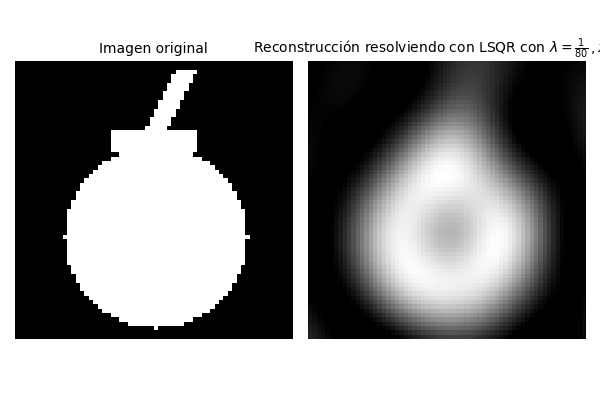
\includegraphics[scale=0.5]{Imagenes/mate_lsqr.png}
	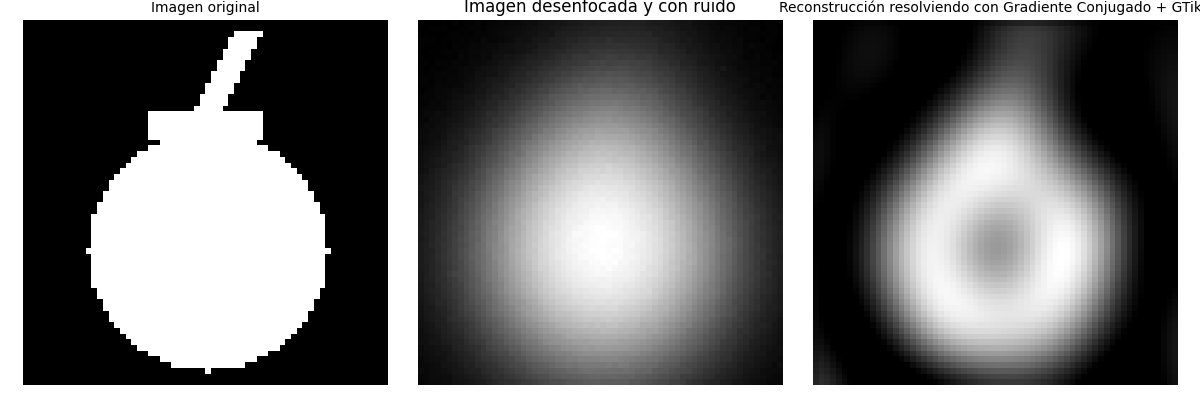
\includegraphics[scale=0.5]{Imagenes/mate_lsmr.png}
	\caption{Reconstrucción de la imagen con ruido usando LSQR y LMSR.\\}
\end{figure}
 
\end{document}
	
